%\section{Dealing with silent data corruption}
Different from crash failures which crashes a processor, silent data corruption allows a faulty processor to continue to completion but may silently generate incorrect results. To deal with $f$ failures, $(2f+1)$ replicas are needed, and voting is required periodically to detect failure. For example, when at most 1 silent data corruption could occur, 3 replicas are sufficient to detect and tolerate the failure. In the following, we will focus on tolerating one silent data corruption per data partition. 

Compared to traditional replication techniques, Shadow Computing can deal with silent data corruption with higher efficiency and less resource requirement. For each partition, Shadow Computing associates 2 fast replicas with 1 slow replica. To save energy, the slow replica executes at a potentially lower rate than the 2 fast replicas, and dynamically speeds up if a fast replica fails. 

To take advantage of the fast progress of the fast replicas, Shadow Computing could perform a leaping at a voting point to leap forward the slow replica. Specifically, when two fast replicas reach a voting point with agreement, the results and execution state are copied to the slow replica to achieve forward progress. This is illustrated in Figure~\ref{fig:silent_model}. If one fast replica fails, the failure will be detected at the next voting point. At this time, the slow replica speeds up to reach the specific voting point and participate in the voting to detect the failed replica. Then a leaping from one correct replica to the failed replica can rejuvenate the failed one, after which all replicas resume normal execution. Note that the slow replica is only useful when one of the fast replicas fails. If the slow replica fails, it will automatically get rejuvenated when the fast replicas reach the next voting point. 

\begin{figure}[!t]
  \begin{center}
      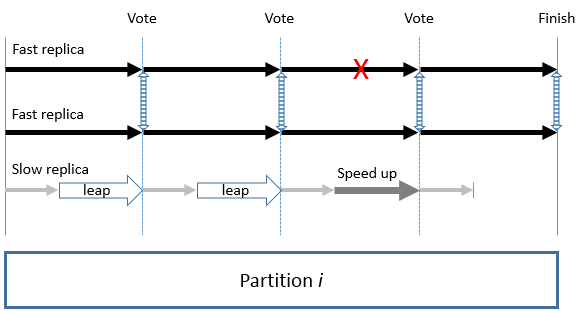
\includegraphics[width=\columnwidth]{figures/silent_model}
  \end{center}
  \vskip -0.1in
  \caption{Tolerating silent data corruption by using two fast replicas with one slow replica.}
  \label{fig:silent_model}
  %\vspace{-0.05in}
\end{figure}

Similar to Section~\ref{sec:crash_collocation}, following subsections develop analytical models for the expected response time and energy consumption, and formulate an optimization framework. (!Explain why didn't consider collocation)

\subsection{Notations}
Let $W$ denote the required workload to process one partition. Let $N$ denote the number of voting points. The voting interval is $w=\frac{W}{N}$. Let $\sigma_{max}$ denote the maximum execution rate. $R_{min}=\frac{W}{\sigma_{max}}$ is the minimal response time. Let $\overline{R}=(1+\alpha)R_{min}$ $(0\leq \alpha \leq 1)$ denote the target response time considering fault tolerance. Let $\lambda$ denote the failure rate, and $f(t)$ denote the failure density function. %Let $d(t)$ denote the failure detection time at a voting point. 
Let $E(\sigma, [t_1, t_2])$ denote the energy consumption of a replica when executing at rate $\sigma$ for an interval from $t_1$ to $t_2$. For each leaping, let $T_l$ denote the time cost, and $E_l$ denote the energy cost.

To deal with silent data corruption, the Shadow Computing model entails three execution rates:
\begin{itemize}
	\item $\sigma_m$, the execution rate of the fast replicas 
    \item $\sigma_b$, the execution rate of the slow replica before a fast replica fails
    \item $\sigma_a$, the execution rate of the slow replica after a fast replica fails
\end{itemize}

\subsection{Response time}
Assuming there is at most one silent data corruption, two scenarios need to be considered, i.e., no fast replica failure, or one fast replica fails. The failure of the slow replica has no impact on the response time. 

In the first scenario, where no failure occurs, the execution time is determined by the fast replicas, as $t_r^m=\frac{W}{\sigma_m}$. Considering the time for leaping, the total response time is $t_{rl}^m=\frac{W}{\sigma_m} + N \times T_l$.

In the second scenario, 
where a fast replica fails, the delay is the time for the slow replica to catch up with respect to a voting interval. The time for a fast replica to complete a voting interval is $t_v = \frac{w}{\sigma_m}$. The time required by the slow replica to complete the remaining work in the current interval is $t_d = \frac{w - t_v\times \sigma_b}{\sigma_a}$. The execution time is $t_r^s = t_r^m + t_d$. Considering the time for leaping, the total response time is $t_{rl}^s=t_r^s + N \times T_l$.
%the response time is determined by the slow replica. The work completed by the slow replica before the fast replicas complete is $w_b = \sigma_b \times t_r^m$. Then the remaining work for the slow replica to complete is $w_a = W - w_b$. As a result, the total response time by the slow replica is $t_r^s = t_r^m + \frac{w_a}{\sigma_a} = \frac{W(\sigma_m + \sigma_a - \sigma_b)}{\sigma_m \sigma_a}$.



\subsection{Energy consumption}
To calculate energy consumption, we also use the power model described in Section~\ref{sec:power_model}.
Corresponding to the two scenarios in the above response time analysis, the energy consumption also falls into two cases. 

If neither of the fast replicas fails, the energy consumption of the three replicas weighted by its probability is
\begin{equation}
\begin{split}
E_1 = & (1 - \int_{0}^{t_r^m} f(t)dt)^2  \times \\
      & \{2E(\sigma_m, [0, t_r^m])+E(\sigma_b, [0, t_r^m])\}
%E_1 = & (1 - \int_{0}^{t_r^m} f_m(t)dt)^2  \times \\
%      & \{2E(\sigma_m, [0, t_r^m])+E(\sigma_b, [0, t_r^m])\}
\end{split}
\end{equation}
The first line is the probability that neither of the fast replicas fails. The second line models the energy of the three replicas during normal execution.

If one fast replica fails, the energy consumption weighted by its probability is 
\begin{equation}
\begin{split}
E_2 = & 2(1 - \int_{0}^{t_r^m} f(t)dt) \times \int_{0}^{t_r^m} f(t)dt \times 
\\  & \{2E(\sigma_m, [0, t_r^m])+E(\sigma_b, [0, t_r^m]) \\ & + 2E(0, [t_r^m, t_r^s])+E(\sigma_a, [t_r^m, t_r^s]\} 
%E_2 = & 2(1 - \int_{0}^{t_r^m} f_m(t)dt) \times \int_{0}^{t_r^m} f_m(t)dt \times 
%\\  & \{2E(\sigma_m, [0, t_r^m])+E(\sigma_b, [0, t_r^m]) \\ & + 2E(0, [t_r^m, t_r^s])+E(\sigma_a, [t_r^m, t_r^s]\} 
\end{split}
\end{equation}
The first line calculates the probability that one fast replica fails while the other successfully completes. In addition to the energy in the first scenario, also accounted is the energy consumed during slow replica catches up, including the fast replicas' idly waiting and the slow replica's speeding up. 



All in all, the total energy consumption is the sum of the above two, plus the energy cost of leaping, i.e., $E_{total}=E_1 + E_2 + N\times E_l$. 

\subsection{Optimization}
\label{sec:silent_opt}
Similar to dealing with crash failures, an optimization problem can be formulated for dealing with silent data corruption to derive the optimal values for the three execution rates, in order to minimize the total energy consumption while meeting response time constraint. 

\begin{equation}
\begin{alignedat}{2}
\min_{\sigma_m,\sigma_s^b,\sigma_s^a} \qquad  & E_{total} (W,N,\overline{R},\rho,\lambda,\sigma_{max}, T_l, E_l)  \\
s.t.  \qquad          & 0 \leq \sigma_m \leq \sigma_{max} \\
                      & 0 \leq \sigma_s^b \leq \sigma_m\\
                      & \sigma_s^b \leq \sigma_s^a \leq \sigma_{max} \\
                      & t_{rl}^s \leq \overline{R}
\end{alignedat}
\end{equation}

The first constraint says the execution rate of the fast replicas should observe the physical processor limit. The second constraint indicates that the initial rate of the slow replica should not exceed that of the fast replicas. The third constraint ensures that the slow replica could speed up after detecting a failure. The last constraint guarantees that the deadline is met even in the case of failure.







